\chapter{Sample Chapter}\label{chap:sample}

Some text with a reference to \fref{sec:sample}.

\section{Sample section}\label{sec:sample}

\begin{figure}[ht]
    \centering
    \begin{subfigure}[b]{0.45\textwidth}
        \centering
        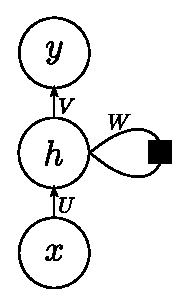
\includegraphics[height=3.2cm]{img/rnn}
        \caption{Description}
        \label{fig:a}
    \end{subfigure}
    ~
    \begin{subfigure}[b]{0.45\textwidth}
        \centering
        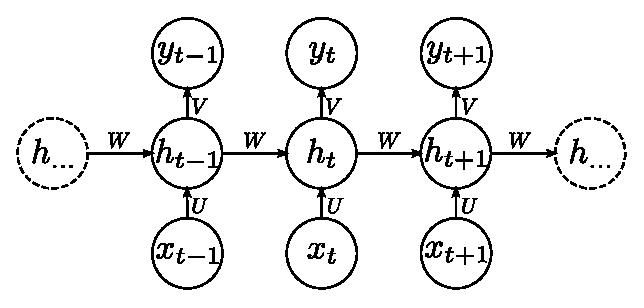
\includegraphics[height=3.2cm]{img/rnn_unfolded}
        \caption{Description}
        \label{fig:b}
    \end{subfigure}
    \caption{Long Description of \fref{fig:a} and \fref{fig:b}. Adapted from~\cite{Goodfellow-et-al-2016}}
    \label{fig:rnns}
\end{figure}

This subsection includes a float containing two figures, as shown in \fref{fig:rnns}. Also, I would like to show off the use of footurls\footurl[It can take additional text]{https://example.com}, which automatically format the URL and add a time stamp.